\documentclass[convert]{standalone}

\usepackage{tikz}
\usepackage{graphicx}
\pagestyle{empty}

% INT_AY22_L01_Fig02_Trinket_fullscreen.png

\begin{document}
\begin{tikzpicture}[> = latex]

	% Screen capture
	
	\node at (0, 0) {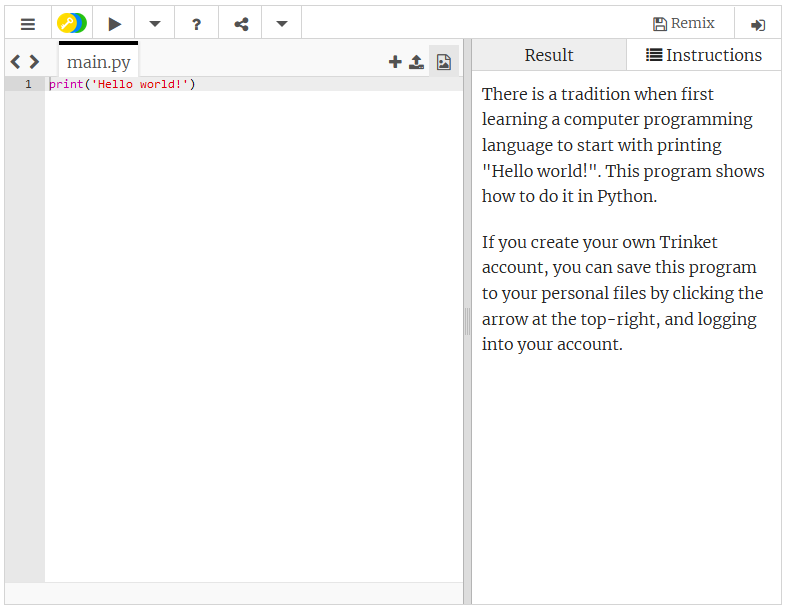
\includegraphics{L01_Hello_world_program.png}};
	
	% Main program
	
	\draw [very thick, red] (-9.2, -7.3) rectangle (1.9, 6.1);
	
	\node (program) [rectangle, fill = green!20, rounded corners, align = center] at (-7, 4) {Area for\\program code};
	\draw [->] (program.west) -- (-9.2, 4);
	
	% Run button
	
	\draw [very thick, red] (-7.4, 7.4) circle (0.5 cm);
	
	\node (run) [rectangle, fill = green!20, rounded corners, align = center] at (-6, 8.5) {Click to run\\program};
	\draw [->] (run.south) to [out = 270, in = 0] (-6.9, 7.4);
	
	% Instructions
	
	\node (info) [rectangle, fill = green!20, rounded corners, align = center] at (5, -2.5) {Brief program guide\\and instructions};
	\draw [->] (info.north east) to [out = 45, in = 315] (6.5, -1);
	
	% Toggle between result, instructions
	
	\node (toggle) [rectangle, fill = green!20, rounded corners, align = center] at (5, 8.5) {Click to\\toggle between\\program output\\and instructions};
	\draw [->] (toggle.south) to [out = 270, in = 60] (4.5, 7);
	\draw [->] (toggle.south east) to [out = 315, in = 180] (7, 6.75);
	
	% Fullscreen option
	
	\draw [very thick, red] (-9.65, 7.4) circle (0.5 cm);
	
	\node (full) [rectangle, fill = green!20, rounded corners, align = center] at (-11, 9) {Click for\\fullscreen\\option};
	\draw [->] (full.south) to [out = 270, in = 180] (-10.2, 7.4);
	
	% Access to Trinket account
	
	\draw [very thick, red] (9.7, 7.4) circle (0.5 cm);
	
	\node (trink) [rectangle, fill = green!20, rounded corners, align = center] at (9.7, 8.9) {Access to\\Trinket account};
	\draw [->] (trink.south) to [out = 270, in = 90] (9.7, 7.9);
	
%	% Grid + labels
%	
%	\draw (-11, -8) grid (11, 8);
%	
%	\foreach \x in {-11, -10, ..., 11}
%		\node [fill = white] at (\x, 0) {\x};
%		
%	\foreach \y in {-8, -7, ..., 8}
%		\node [fill = white] at (0, \y) {\y};

\end{tikzpicture}
\end{document}